\begin{figure}[!h]
\chapter{Class Diagrams and Interface Specifications}
\section{Financial Adaptor Class Diagram}
\centering
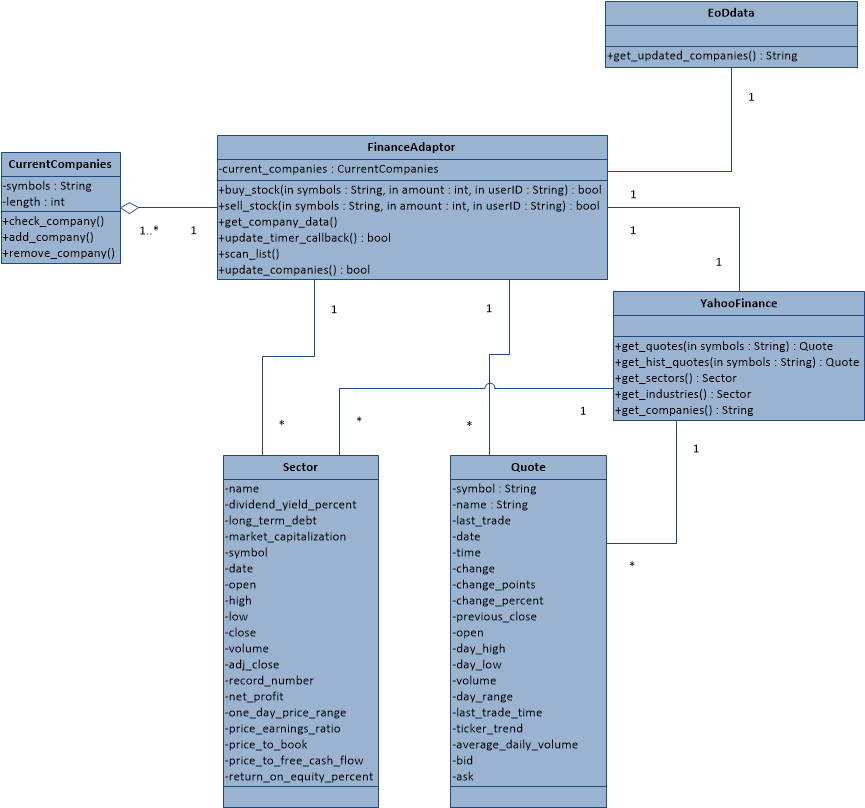
\includegraphics[width=5.5in]{./Diagrams/DomainModel/Financialdomainmodel.png}
\end{figure}

\clearpage

\section{Financial Adaptor Data Types and Operation Signatures}
\subsection{Finance Adaptor}
{\bfseries Attributes} \\*
Our Finance Adaptor performs the functions of validating user queries with 
existing stock symbols, companies, and/or sectors, then mediating between
the Capital Games web server and Yahoo! Finance, enabling our fantasy league
to be playable in real time.  To accomplish data validation, a portion of the
Capital Games database is updated regularly to keep our fantasy stock market
league up to date based off of EODData, an API allowing for the reference to
an up-to-date list of all stock-symbols, company names, and sector/industries. \\* \\*
{\bfseries --- current\_companies : CurrentCompanies } \\*
	This is a reference to a database table updated via an external website, EoDdata,
	that verifies user queries with actual stock symbols, and/or 
	company/sector/inddustry names depending on the user query. \\*\\*

{\bfseries Methods} \\*
Most methods are boolean, returning either success or failure regardng data retrieval.
All other methods are voids, with no arguments, used for executing a specific function. \\* \\*
{\bfseries + buy\_stock (in symbols : String, in amount : int, in userID : String) : bool } \\*
	Method called to buy stock; a typical method that would require the user to query
	up-to-date stock market information via our adaptor. \\*
{\bfseries + sell\_stock (in symbols : String, in amount : int, in userID : String) : bool } \\*
	Method called to sell stock; a typical method that would require the user to query
	up-to-date stock market information via our adaptor. \\*
{\bfseries + get\_company\_data() } \\* 
	This method returns all information available on Yahoo! Finance regarding a user's queried 
	stock. \\*
{\bfseries + update\_timer\_callback() : bool } \\*
	An internal timer signaling the stock query from Yahoo! Finance.  \\*
{\bfseries + scan_list()  }\\*
	This method checks against the Capital Games' database. \\*
{\bfseries + update\_companies() : bool } \\*

	This method updates the information in the Caital Games' database from both Yahoo! Finance
	and EODData. \\*
\subsection{Current Companies}
 

{\bfseries Attributes} \\*
Current Companies is the database table that our Finance Adaptor actually checks against 
when validating user queries. At a regular interval (based on method update_timer_callback from
the Finance Adaptor, the Finance Adaptor retrieves data from EODData to update the Current 
Companies database table.) This is done to maximize efficiency by minimizing the amount of time
the adaptor must retrieve data from EODData. \\* \\*
{\bfseries --- symbols : String \\* }
	This is all stock symbols. \\* 
{\bfseries --- length : integer \\* }
	This defines how many total stock symbols are on the list. \\* 


{\bfseries Methods} \\*
All of these methods are invoked after the stock symbol or company name has been validated.
All methods perform queries regarding updating the Current Companies tabe. \\* \\* 
{\bfseries + check\_company () } \\*
	This method returns all informaton regarding a stock, to be parsed by the Finance Adaptor to
	retrieve what the user is querying for. \\*
{\bfseries + add\_company () } \\*
	Method called to add a company to the database in cases such as Initial Public Offering of
	shares. \\*
{\bfseries + remove\_company() } \\*
	Method called to remove a company from the database in case of acquisition. \\*

\subsection{EODData}
{\bfseries Attributes}  
EODData is an external web app, much like Yahoo! Finance, that contains data regarding stocks
in bulk. Essentially we are using it to validate stock user queries as it enables us to have a
database of all stock symbols and company names. \\* \\*

{\bfseries Methods} \\* \\*
{\bfseries + get\_updated\_companies ()} \\*
	This method updates the Current Comapnies database table based on the EODData API. \\*

\subsection{Yahoo! Finance} 
{\bfseries Attributes}  \\*
Yahoo! Finance is the main external API we are utilizing for up-to-date stock market information
for our fantasy stock market league. It is highly reliable and enables to make several, serparate
queries of individual or multiple stocks at once. \\* \\*

{\bfseries Methods} \\* \\*
{\bfseries + get\_quotes(in symbols : String) : Quote   } \\*
	This method returns quotes from a stock symbol based on Yahoo! Finance.
{\bfseries + get\_hist\_quotes(in symbols : String) : Quote   } \\*
	This method returns historical quotes from a stock symbol based on Yahoo! Finance that
	spans a larger period of time a user may draw specific information from in a predefined
	period of time. \\*
{\bfseries + get\_sectors() : Sector  } \\*
	Gets information similar to quotes on a financial sector \\*
{\bfseries + get\_industries() : Sector   } \\*
	Get information in industries that fall under financial sectors. \\*
{\bfseries + get\_companies() : String  } \\*
	Retrieves all company information from Yahoo! Finance. \\*

\subsection{Sector}
{\bfseries Attributes} \\*
US Market Sectors are essentially an umbrella category for certain groups of stocks.
For example, technology stocks such as Google and Microsoft would belong to the
technology sector. These have attributes similar to a stock quote. Essentially
all attributes are the stock information one would find searching the sector on
Yahoo! Finance. 

\subsection{Quote}
{\bfseries Attributes} \\*
Quotes will essentially return a list of all data that has been retrieved from
Yahoo! Finrance, similar to above.

\section{Financial Adaptor Traceability Matrix}

{
\begin{centering} % Aligns center 
\begin{tabular}{|c||c|c|c|c|c|}
\hline
Class
& \rotatebox{90}{Finance Adaptor}
& \rotatebox{90}{Current Companies}
& \rotatebox{90}{EODData}
& \rotatebox{90}{Yahoo! FInance} \\
\hline
Finance Adaptor & X &  &  &  \\
\hline
Current Companies & X & X & X &  \\
\hline
EODData &  &  & X &  \\
\hline
Yahoo Finance &  &  &  & X \\
\hline
Sector & X &  &  & X \\
\hline
Quote & X &  &  & X \\
\hline
\end{tabular}
\end{centering}
}

Our Financial Adaptor practically handles all querying of data. As a result, most classes trace
to the Financial Adaptor. While EODData and Yahoo! Finance are external to the database in which 
all items subordinate to the Financial Adaptor exists, the fact that our FInancial Adaptor 
queries them for data validation and retrieval makes them essential conceptual entities in our
Traceability Matrix. 

For example, sectors and Quotes as mapped to the Financial Adaptor exist in their
original form inside Yahoo! Finance's respective APIs, hence they map to Yahoo! Finance. Also, Current Companies is also a database table queried by
the Financial Adaptor and updated via EODData, hence it maps to both 
the Financial Adaptor and EODData.

\subsection{Object Constraint Language}
In order to separate ideas in OCL, we will split it up descriptions by each class in the class diagram.
\subsubsection{Finanace Adaptor Class}
In this class, we have a few constraints that deal with this class being kind of central to all of the other classes that make up our financial adaptor. The function to buy or sell stocks are the same in their constraints. You must have a symbol name which is not equivalent to NULL and is the symbol of a company that exists. The amount must be a positive integer and if you are buying you must have enough to spend on this. Lastly, the userID must be plugged in, so that must also not be NULL and it should hold the username of someone who exists. The function get\_company\_data must have a symbol passed in that exists and is not NULL. The function scan\_list must be called after the list already exists, or there will be an error. Lastly, the update\_companies function must have a return from EoDdata that is valid and not corrupted.
\subsubsection{Current Companies}
All three of the functions in this class have the same constraint, that the symbol passed in must exist. On top of that, the ``length'' variable must always be equal to the amount of symbols in the ``symbols'' variable.
\subsubsection{Yahoo! Finanace Class}
Fortunately for us, this is another simple addition for it is dealt with completely by Yahoo! Finance. Something that we do have to be careful of is making sure that if we are calling the get\_quotes or get\_hist\_quotes, we have to make sure that we are passing in a valid string. For example, if we passed in a NULL string, we would have an error returned.
\subsubsection{EoDdata Class}
This is the simplest class out of any of the ones we deal with, as there are no variables and only one function that returns a large list of stocks without us having to pass in anything. No constraints in this class.
\subsubsection{Sector and Quote Class}
The constraints on these classes will work as long as Yahoo! Finanace returned results that are valid. These results are checked in the Finance Adaptor Class, and if it did make it past that point, the data that is passed in is fine, and therefore there are no actual constraints on these classes.


\section{Design Patterns}
Various standard design patterns were utilized to provide functionality for things such as authentication, efficient page rendering and object modeling.
\subsection{Model-View-Controller}
The Model-View-Controller (MVC) pattern was heavily used throughout the CapitalGames system to properly organize model logic, business logic and presentation logic. This very intuitive pattern allowed the team to easily delegate work on different levels of the system. Frequently, a selection of team members would develop front-end functionality which required only the views to be altered, while other members implemented backend functionality which was done either in controllers or models. This pattern resulted in a more efficient development lifecycle overall, while also providing some performance gains. Namely, the MVC pattern calls on resources only when they are actually needed which prevents unnecessary overhead. For example, methods developed to be called only programmatically don't attempt to display a view which results in faster responses.
\subsection{Security Proxy}
The security proxy pattern was the core of our secure authentication system. This proxy pattern allowed us to easily protect content based on user role or other variables. The security proxy was implemented very similarly to that described in the textbook. Particularly, it behaved as a transparent filter between an HTTP request and a controllers method. Authentication requirements could easily be chained onto each other making it possible to create custom controller prerequisites. Finally, because the security proxy filtered every request made on a controller instead of just requests made upon login, all sensitive features of the site had a very robust shell which no user could easily bypass. This improved our design by providing solid, system-wide security.
\subsection{ActiveRecord Pattern}
The ActiveRecord pattern, an intelligent implementation of a database access design pattern, was used exclusively to interact with persistant storage technologies used in the CapitalGames system. This pattern offered the major advantage of not needing to hard code any database-specific queries. All requests made to the ActiveRecord Pattern are translated to the currently used DB system's language and data is returned in directly its object form. The lack of need to write direct queries also lead to a great side effect, namely database agnosticism which allowed various database implementations to be used during different stages of development. During developmnt SQLite was used for its lightweight footprint on the developers machine, then for production MySQL was used as it is considerably more efficient when dealing with larger amounts of data. This design certainly improved our development by saving countless hours of development time.
\subsection{RESTful Design}
The RESTful design pattern being used more and more now on the web allowed us to implement our asynchronous order processing system. The RESTful design of some internal functionality allowed it to be accessed programmatically and securily through a simple API. As RESTful services are at the heart of Ruby on Rails, it did not require a lot of effort to expose some internal functionality without creating major security holes. Future iterations of CapitalGames will continue to rely on the stateful communication that our RESTful API offers.
\subsection{Responsive UI Pattern}
The Bootstrap UI framework implemented a design pattern completely segregating visual presntation from content and user experience. This provided in a beautiful responsive design which adapted to different client devices ranging from desktops to smartphones. The pattern takes advantage of the flexible markup of HTML5 to customize it on the fly when the page is rendering in the browser using Javascript and CSS. This allowed our team to target the rapidly growing mobile users without much extra implemetation effort. It also inherently produced a faster user experience since minimal processing is done during initial page rendering and mostly done asynchronously once the page is already viewable to the user. We actively strived to achieve both of these goals.
